\documentclass[12pt,a4paper]{article}

\usepackage{amsmath}
\usepackage{graphicx}
\usepackage{geometry}
\geometry{margin=1in}

\begin{document}
\noindent
\begin{minipage}{0.6\textwidth}

\includegraphics[width=0.75\textwidth]{IIITB-COMET-Logo.png}
\end{minipage}
\begin{minipage}{0.38\textwidth}
\begin{flushright}
\textbf{DARSI VAMSI}
\newline
\textbf{COMET FWC 071}
\end{flushright}
\end{minipage}





The objective of this experiment is to analyze a combinational logic circuit, simplify the obtained Boolean expression, and verify the output through hardware implementation using Arduino.
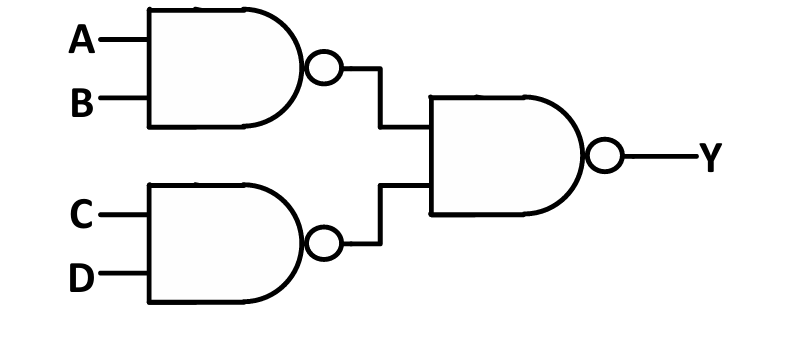
\includegraphics[width=0.75\textwidth]{figure.png}
\newline

\begin{equation}
\boxed{Y=AB+CD}
\end{equation}

\section{Hardware Requirements}

\begin{enumerate}
\item Arduino Uno
\item Common Anode Seven Segment Display
\item Breadboard
\item Jumper Wires
\item 220 $\Omega$ Resistors
\item Android Device with Termux and PlatformIO
\end{enumerate}

\section{Circuit Connections}

\begin{table}[h]
\centering
\begin{tabular}{|c|c|}
\hline
Segment & Arduino Pin \\
\hline
a & D2 \\
\hline
b & D3 \\
\hline
c & D4 \\
\hline
d & D5 \\
\hline
e & D6 \\
\hline
f & D7 \\
\hline
g & D8 \\
\hline
COM & +5V \\
\hline
\end{tabular}
\caption{Seven Segment Connections}
\end{table}

The common anode terminals of the display are connected to +5V.

\section{Implementation}

The Boolean expression
\begin{equation}
[
Y=AB+CD
]
\end{equation}
was implemented in Arduino using predefined input combinations.

The output obtained from the logic expression was displayed on the Common Anode Seven Segment Display.

Two test cases were considered:

\begin{itemize}
\item Input Set 1: $A=1,\\ B=1,\\ C=0,\\ D=0$
\item Input Set 2: $A=0,\\ B=1,\\ C=0,\\ D=1$
\end{itemize}

For Input Set 1,

\begin{equation}
Y=(1)(1)+(0)(0)=1
\end{equation}

The display shows digit 1.

For Input Set 2,

\begin{equation}
Y=(0)(1)+(0)(1)=0
\end{equation}

The display shows digit 0.

\section{Observation}

\begin{table}[h]
\centering
\begin{tabular}{|c|c|c|c|c|}
\hline
A & B & C & D & Y=AB+CD \\
\hline
0 & 0 & 0 & 0 & 0 \\
0 & 0 & 0 & 1 & 0 \\
0 & 0 & 1 & 0 & 0 \\
0 & 0 & 1 & 1 & 1 \\
0 & 1 & 0 & 0 & 0 \\
0 & 1 & 0 & 1 & 0 \\
0 & 1 & 1 & 0 & 0 \\
0 & 1 & 1 & 1 & 1 \\
1 & 0 & 0 & 0 & 0 \\
1 & 0 & 0 & 1 & 0 \\
1 & 0 & 1 & 0 & 0 \\
1 & 0 & 1 & 1 & 1 \\
1 & 1 & 0 & 0 & 1 \\
1 & 1 & 0 & 1 & 1 \\
1 & 1 & 1 & 0 & 1 \\
1 & 1 & 1 & 1 & 1 \\
\hline
\end{tabular}
\caption{Truth Table for $Y = AB + CD$}
\end{table}

The output displayed on the seven segment display matched the result obtained from the Boolean expression.
\newpage
\section{Result}

The Boolean function

\begin{equation}
{Y=AB+CD}
\end{equation}

was successfully implemented using Arduino Uno and a Common Anode Seven Segment Display.\newline
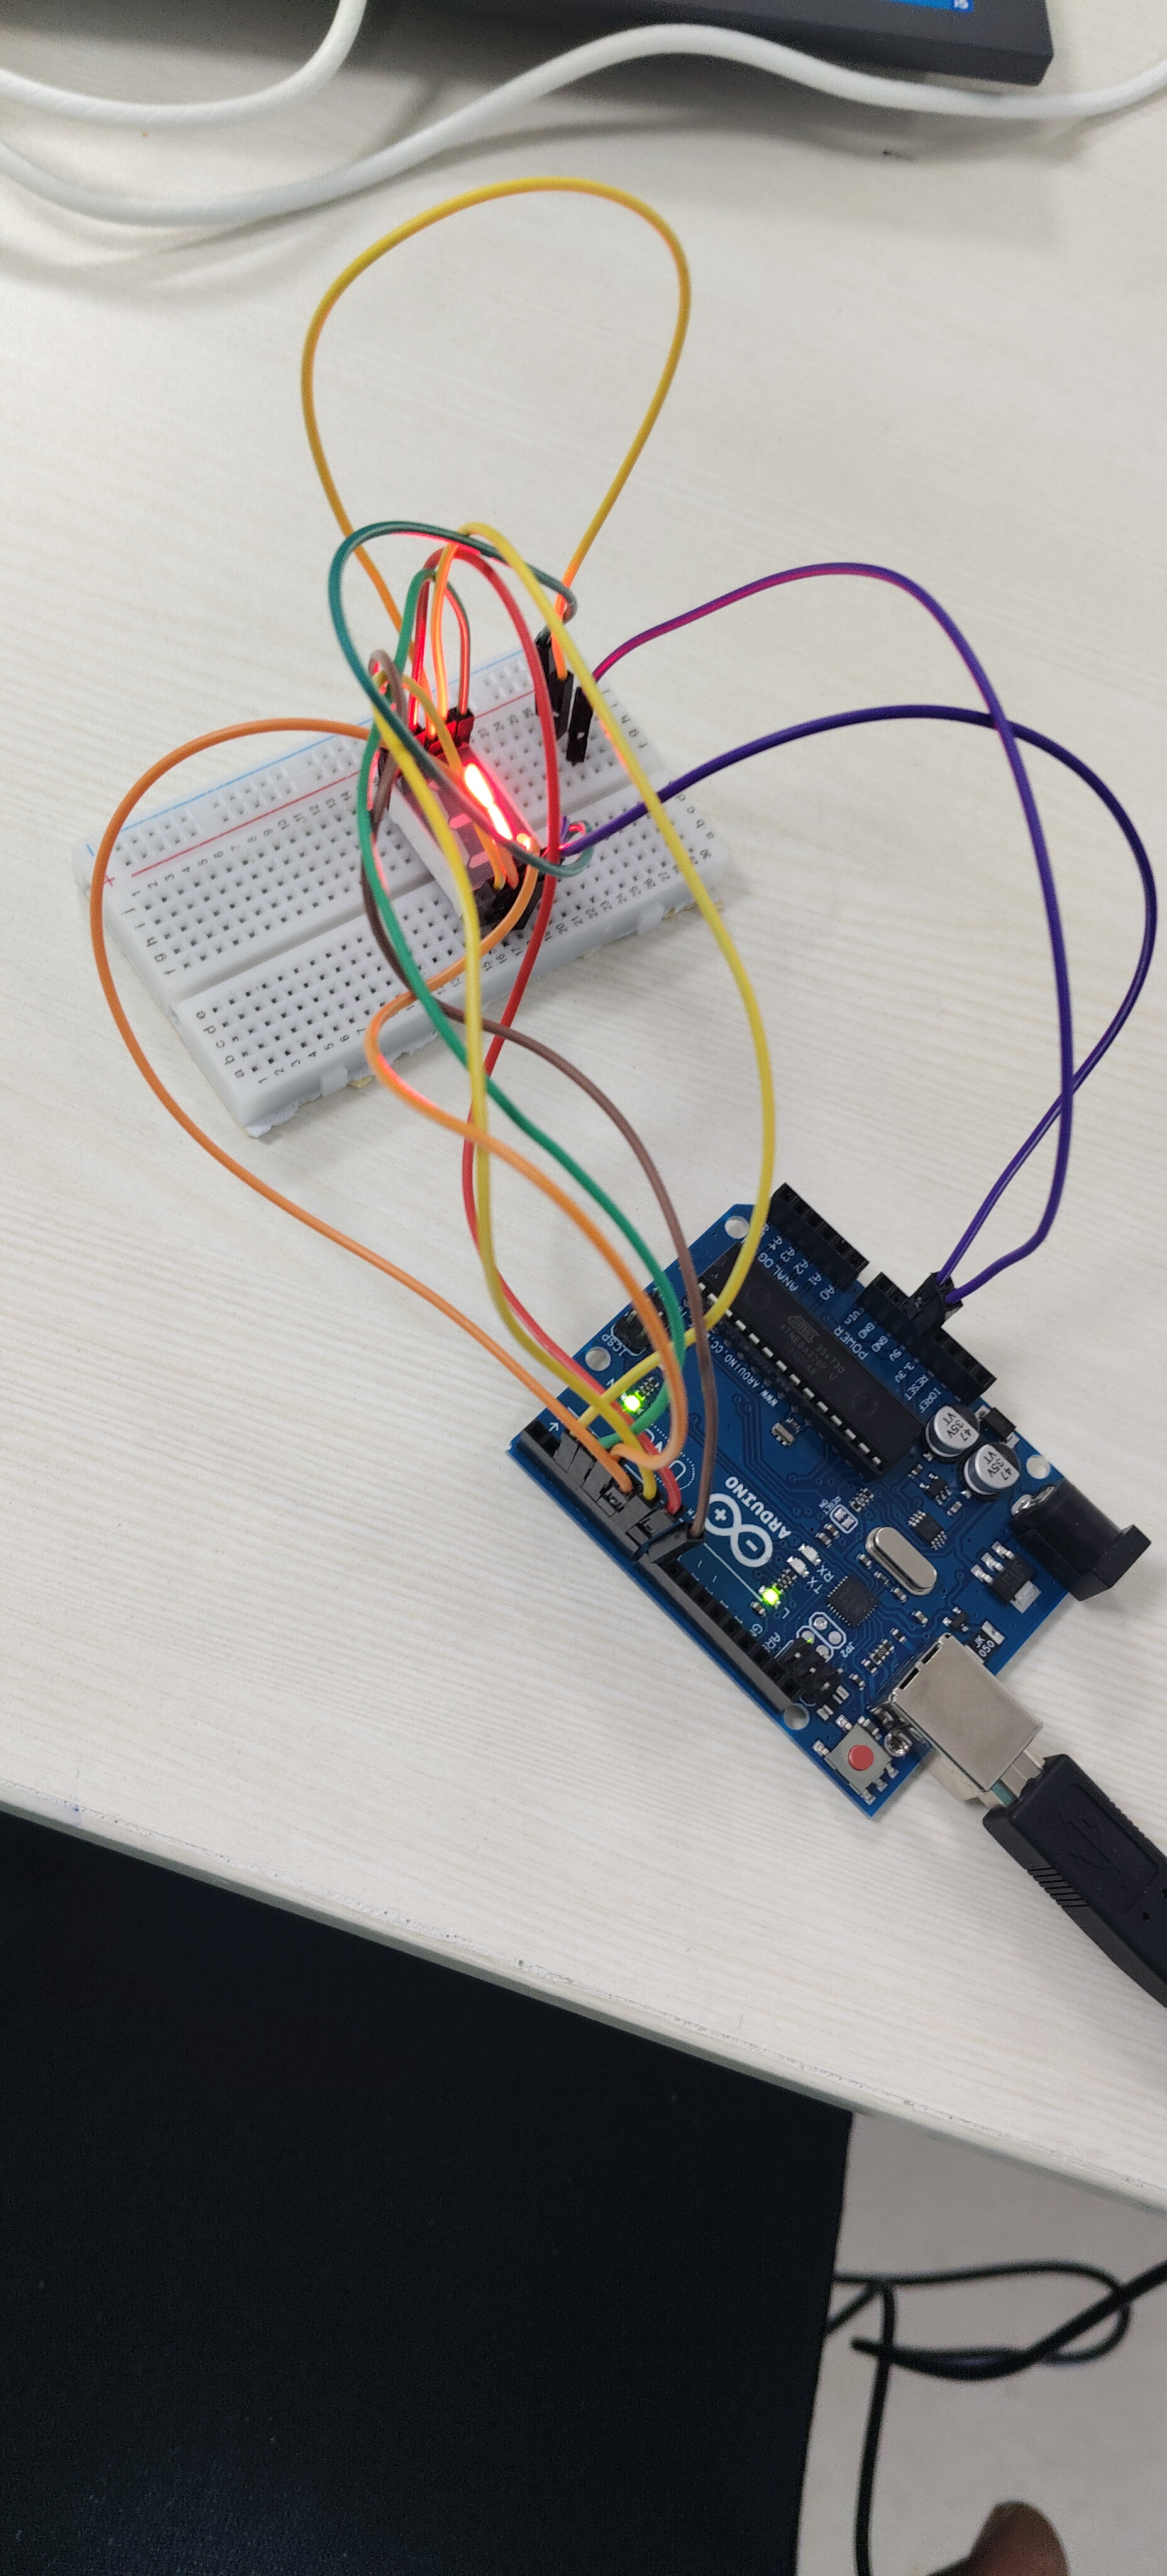
\includegraphics[width=0.75\textwidth]{7seg.jpeg}


\end{document}
